% Chapter Template

\chapter{Ensayos y resultados} % Main chapter title
En este capítulo se explican las pruebas realizadas al hardware, firmware, controladores y a la plataforma IoT.
\label{Chapter4} % Change X to a consecutive number; for referencing this chapter elsewhere, use \ref{ChapterX}

%----------------------------------------------------------------------------------------
%	SECTION 1
%----------------------------------------------------------------------------------------

\section{Pruebas unitarias}
Para la implementación de los drivers se utilizó la metodología de desarrollo TDD. Esto implica que se escribieron pruebas unitarias para los drivers. Se utilizó ceedling como herramienta de desarrollo de pruebas automáticas.

En el código \ref{cod:codigo test driver AHT10} se muestra la prueba implementada para la función de \emph{aht10\_get\_status()} del driver del sensor AHT10. Internamente utiliza funciones mock para la lectura y escritura por protocolo I2C, líneas 6,11 y 15. Se prueban dos casos: cuando la lectura de los registros es 0 y cuando es 255.
\begin{lstlisting}[label=cod:codigo test driver AHT10,caption=Tests del driver del sensor AHT10.]
//Prueba de funcion para obtener el estado del sensor AHT10
void test_estado_del_sensor(void)
{
  uint8_t buffer[1]={0};
  uint8_t data=0;
  read_I2C_STM32L432_port_ExpectAndReturn(AHT10_ADDRESS_SLAVE,buffer,1,AHT10_OK);
  read_I2C_STM32L432_port_ReturnThruPtr_buffer(&data);
  TEST_ASSERT_EQUAL(SENSOR_IDLE,aht10_get_status(&aht10config));
  
  data=255;
  read_I2C_STM32L432_port_ExpectAndReturn(AHT10_ADDRESS_SLAVE,buffer,1,AHT10_OK);
  read_I2C_STM32L432_port_ReturnThruPtr_buffer(&data);
  TEST_ASSERT_EQUAL(SENSOR_BUSY,aht10_get_status(&aht10config));
  
  read_I2C_STM32L432_port_ExpectAndReturn(AHT10_ADDRESS_SLAVE,buffer,1,AHT10_ERROR);
  TEST_ASSERT_EQUAL(SENSOR_BUSY,aht10_get_status(&aht10config)); 
}
\end{lstlisting}

En el código \ref{cod:codigo test driver bg96} se muestra la prueba desarrollada para la función \emph{send\_sms\_bg96()} encargada de mandar los mensajes de texto del driver BG96. Se probaron varios casos, cuando la función de envío de comandos responde con un OK y cuando responde con errores.
\begin{lstlisting}[label=cod:codigo test driver bg96,caption=Tests del driver del modulo bg96.] 
//Prueba de la funcion para mandar sms  
void test_send_sms_bg96(void)
{
  char buffer_resp[30]={0};
  send_data_ExpectAndReturn("AT+CMGS=\"72950576\"\r",RS_BG96_SIGNAL,buffer_resp,12000,FT_BG96_OK);
  send_data_ExpectAndReturn("HOLA\x1a\r",RS_BG96_OK,buffer_resp,12000,FT_BG96_OK);
  TEST_ASSERT_EQUAL(FT_BG96_OK,send_sms_bg96(&config_module,"72950576","HOLA"));

  send_data_ExpectAndReturn("AT+CMGS=\"72950576\"\r",RS_BG96_SIGNAL,buffer_resp,12000,FT_BG96_ERROR);
  TEST_ASSERT_EQUAL(FT_BG96_ERROR,send_sms_bg96(&config_module,"72950576","HOLA"));

  send_data_ExpectAndReturn("AT+CMGS=\"72950576\"\r",RS_BG96_SIGNAL,buffer_resp,12000,FT_BG96_OK);
  send_data_ExpectAndReturn("HOLA\x1a\r",RS_BG96_OK,buffer_resp,12000,FT_BG96_ERROR);
  TEST_ASSERT_EQUAL(FT_BG96_ERROR,send_sms_bg96(&config_module,"72950576","HOLA"));
}
\end{lstlisting}

Una forma cuantitativa de evaluar estas pruebas son los informes de cobertura generados por ceedling.

En la figura \ref{fig:Cobertura aht10} se puede observar el informe de cobertura del driver aht10, donde se puede apreciar que las pruebas ejecutan el 100\% de las líneas de código escritas y explora el 100\% de las combinaciones en los saltos de condicionales.

En la figura \ref{fig:Cobertura BG96} también se observa el informe de cobertura del driver de bg96, con 98.4\% de líneas ejecutadas y explora más del 98.3\% de combinaciones posibles. 

\begin{figure}[h!]
    \centering
      \includegraphics[width=\linewidth, height=4cm]{./Figures/cobertura_aht10.png}
    \caption{Informe de cobertura driver aht10.}
      \label{fig:Cobertura aht10}
  \end{figure}

\begin{figure}[h!]
    \centering
      \includegraphics[width=\linewidth, height=4cm]{./Figures/cobertura_bg96.png}
    \caption{Informe de cobertura driver BG96.}
      \label{fig:Cobertura BG96}
\end{figure}

\section{Pruebas de la plataforma IoT}
\subsection{Prueba de inyección de mensajes}
El objetivo de la prueba de inyección de mensajes a la plataforma IoT, es verificar la llegada de los mensajes mandados por un cliente MQTT al broker de ThingsBoard.
Para realizar el envío de datos al broker, se utilizó el programa mosquitto. Para realizar esta prueba se ejecutó el comando de mosquitto que se muestra en la figura \ref{fig:mosquitto pub}.

\begin{figure}[h!]
  \centering
    \includegraphics[width=\linewidth, height=3cm]{./Figures/mosquito_enviodatos.png}
  \caption{Envio de datos por el cliente MQTT de mosquitto.}
    \label{fig:mosquitto pub}
\end{figure}

Donde:
\begin{itemize}
  \item -h dirección del broker
  \item -t tópico 
  \item -u token
  \item -m mensaje en formato json
\end{itemize}

Al ejecutar el comando de la figura \ref{fig:mosquitto pub}, el cliente de mosquitto primeramente se conecta al broker MQTT, luego publica el mensaje en el tópico y finalmente, se desconecta del servidor.

Para comprobar la llegada de los datos al broker de ThingsBoard, se tiene que ir a la sección dispositivos, seleccionar el dispositivo al que se le envio los datos y entrar a la pestaña de última telemetría. En la figura \ref{fig:tb recepcion} podemos ver que los datos enviados llegan correctamente.

\begin{figure}[h!]
  \centering
    \includegraphics[width=5cm, height=6.5cm]{./Figures/tb_recepcion.png}
  \caption{Recepción de datos en el broker MQTT.}
    \label{fig:tb recepcion}
\end{figure}

\subsection{Prueba de la tabla de alarmas del panel visualización}
ThingsBoard permite configurar alarmas con respecto a las variables monitoreadas por el sistema. En el panel de visualización de cada sensor se tiene una tabla de alarmas, que muestra las notificaciones de las alarmas que se activaron.
En la figura \ref{fig:alarmas tb} podemos ver la notificación de una alarma cuando la temperatura ambiente sobrepasa los 43\textcelsius.

\begin{figure}[h!]
  \centering
    \includegraphics[width=\linewidth, height=7cm]{./Figures/alarmas_tb.png}
  \caption{Tabla de alarmas activas.}
    \label{fig:alarmas tb}
\end{figure}

\subsection{Prueba del widget de mapa}
En los paneles de visualización tenemos mapas que muestran la ubicación del dispositivo implementado.
En la figura \ref{fig:map thingsboard}  podemos ver la ubicación del prototipo implementado para el trabajo.

\begin{figure}[h!]
  \centering
    \includegraphics[width=10cm, height=6.5cm]{./Figures/map.png}
  \caption{Ubicación del nodo sensor implementado.}
    \label{fig:map thingsboard}
\end{figure}

\subsection{Prueba de persistencia de datos}
Para realizar la prueba de persistencia de datos, se configuró las gráficas de los paneles de visualización con un entorno de tiempo más amplio.
En las gráficas se estableció un rango de tiempo de 7 días. El resultado se muestra en la figura \ref{fig:Persistencia de datos}.

\begin{figure}[h!]
  \centering
    \includegraphics[width=10cm, height=6cm]{./Figures/persistencia_datos.png}
  \caption{Persistencia de datos.}
    \label{fig:Persistencia de datos}
\end{figure}

\section{Pruebas de hardware}
\subsection{Prueba de comunicación entre el sensor AHT10 y el microcontrolador}
Para comprobar la comunicación por I2C entre el sensor y el microcontrolador se utilizó un analizador lógico.
En la figura \ref{fig:write aht10} podemos ver la trama capturada por el analizador lógico cuando el firmware escribe en un registro del sensor. 

En la figura \ref{fig:read aht10} tenemos la trama capturada cuando se leen los registros del sensor. Se obtienen 6 bytes en los que se encuentra la información de la humedad y la temperatura.


\begin{figure}[h!]
  \centering
    \includegraphics[width=\linewidth, height=3.2cm]{./Figures/write_i2c.png}
  \caption{Trama de escritura al sensor AHT10.}
    \label{fig:write aht10}
\end{figure}

\begin{figure}[h!]
  \centering
    \includegraphics[width=\linewidth, height=3.5cm]{./Figures/read_i2c..png}
  \caption{Trama de lectura del sensor AHT10.}
    \label{fig:read aht10}
\end{figure}

\subsection{Prueba de comunicación entre el módulo BG96 y el microcontrolador}

Para probar la comunicación del microcontrolador con el módulo bg96, se utilizó un analizador lógico, que nos permite ver los comandos que envía el microcontrolador y la respuestas del módulo a estos comandos por protocolo serial.
En la figura \ref{fig:trama uart1} vemos dos canales del analizador  lógico: el canal 2 muestra un comando mandado por el microcontrolador al módulo de comunicación y en el canal 3 la respuesta del módulo al comando enviado.

\begin{figure}[h!]
  \centering
    \includegraphics[width=\linewidth, height=3.5cm]{./Figures/trama_uart1.png}
  \caption{Envío y recepción de comandos por puerto UART.}
    \label{fig:trama uart1}
\end{figure}

\section{Pruebas funcionales del sistema}
Para realizar las pruebas funcionales de todo el sistema, se implementó el prototipo en un cultivo agrícola como se muestra en la figura \ref{fig:implementacion del prototipo}.

\begin{figure}[h!]
  \centering
    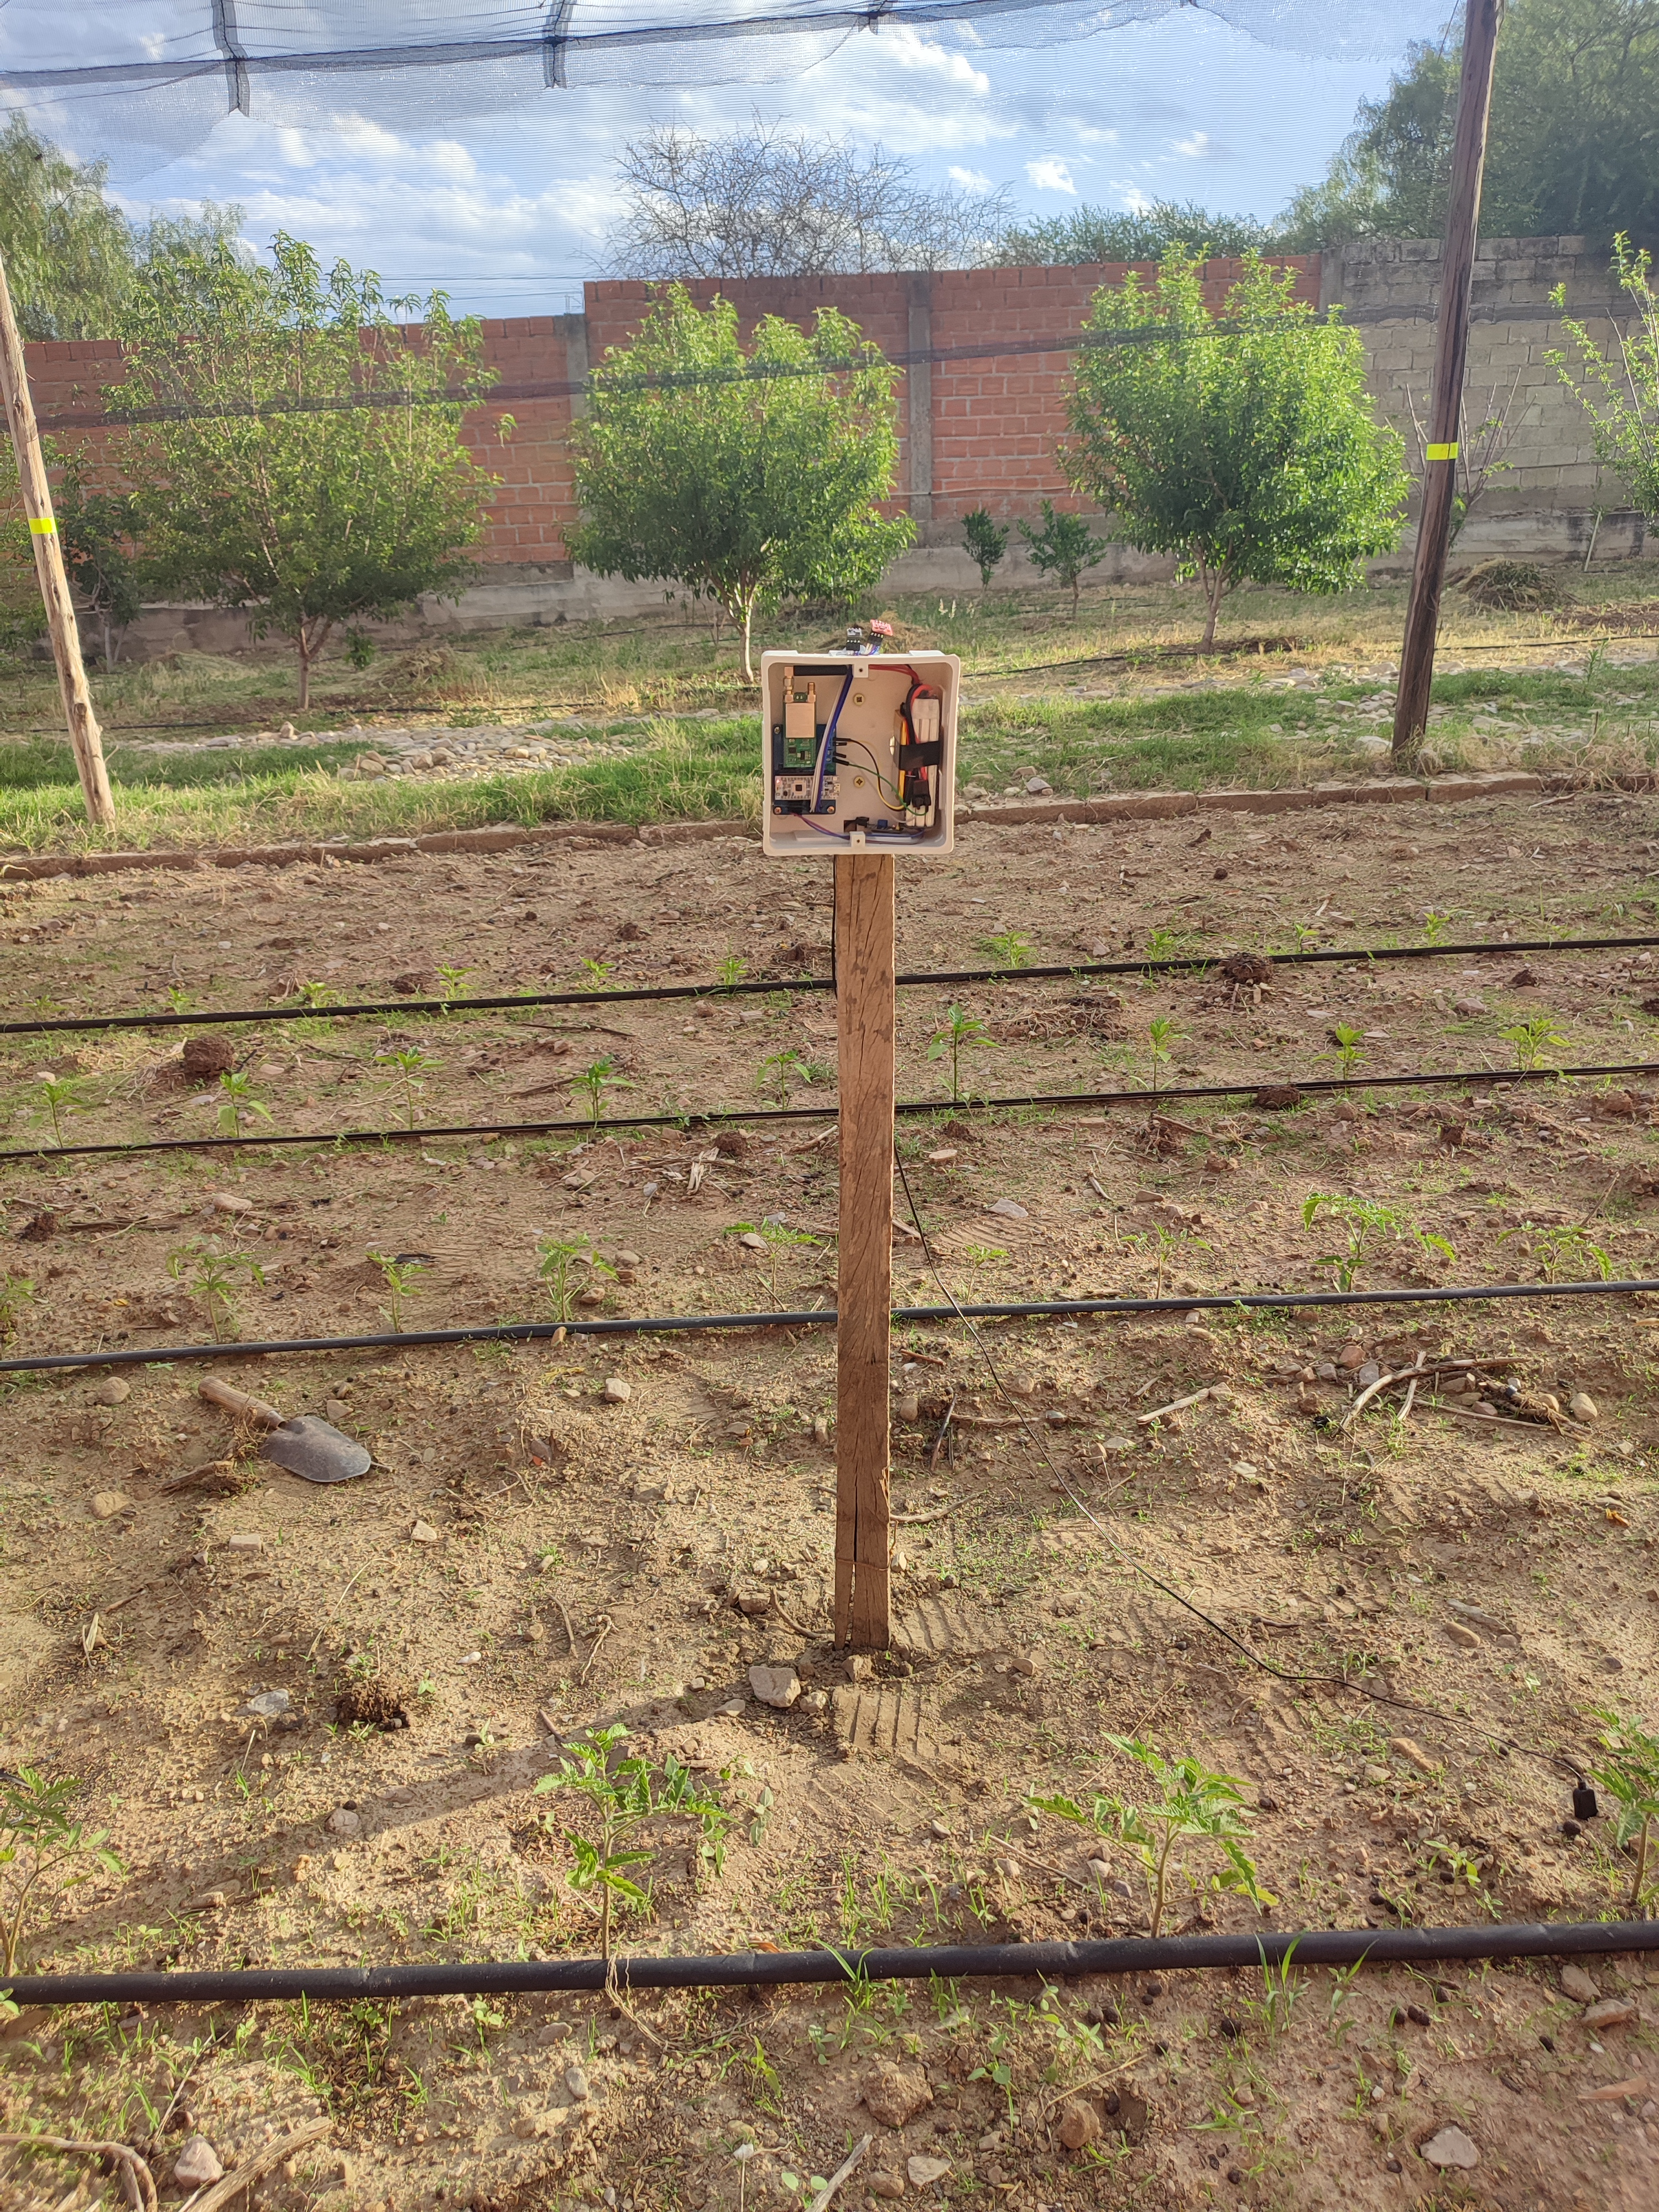
\includegraphics[width=5cm, height=7cm]{./Figures/prot_implementacion.jpg}
  \caption{Implementación del prototipo.}
    \label{fig:implementacion del prototipo}
\end{figure}

\subsection{Pruebas de lectura de los sensores}
Se realizaron varias pruebas al prototipo en diferentes escenarios a continuación se desarrollaran algunas de las pruebas realizadas.
\subsubsection{Prueba uno}
La prueba consistió en realizar la lectura de los sensores en un momento donde se tenían las siguientes condiciones:
\begin{itemize}
  \item Tierra con poca humedad
  \item Temperatura ambiente alta 
  \item Horario de la lectura: 3 p.m
\end{itemize}
En la figura \ref{fig:Condicionales ambientales prueba 1} se puede apreciar las condiciones ambientales en el momento de la prueba.
\begin{figure}[h!]
  \centering
    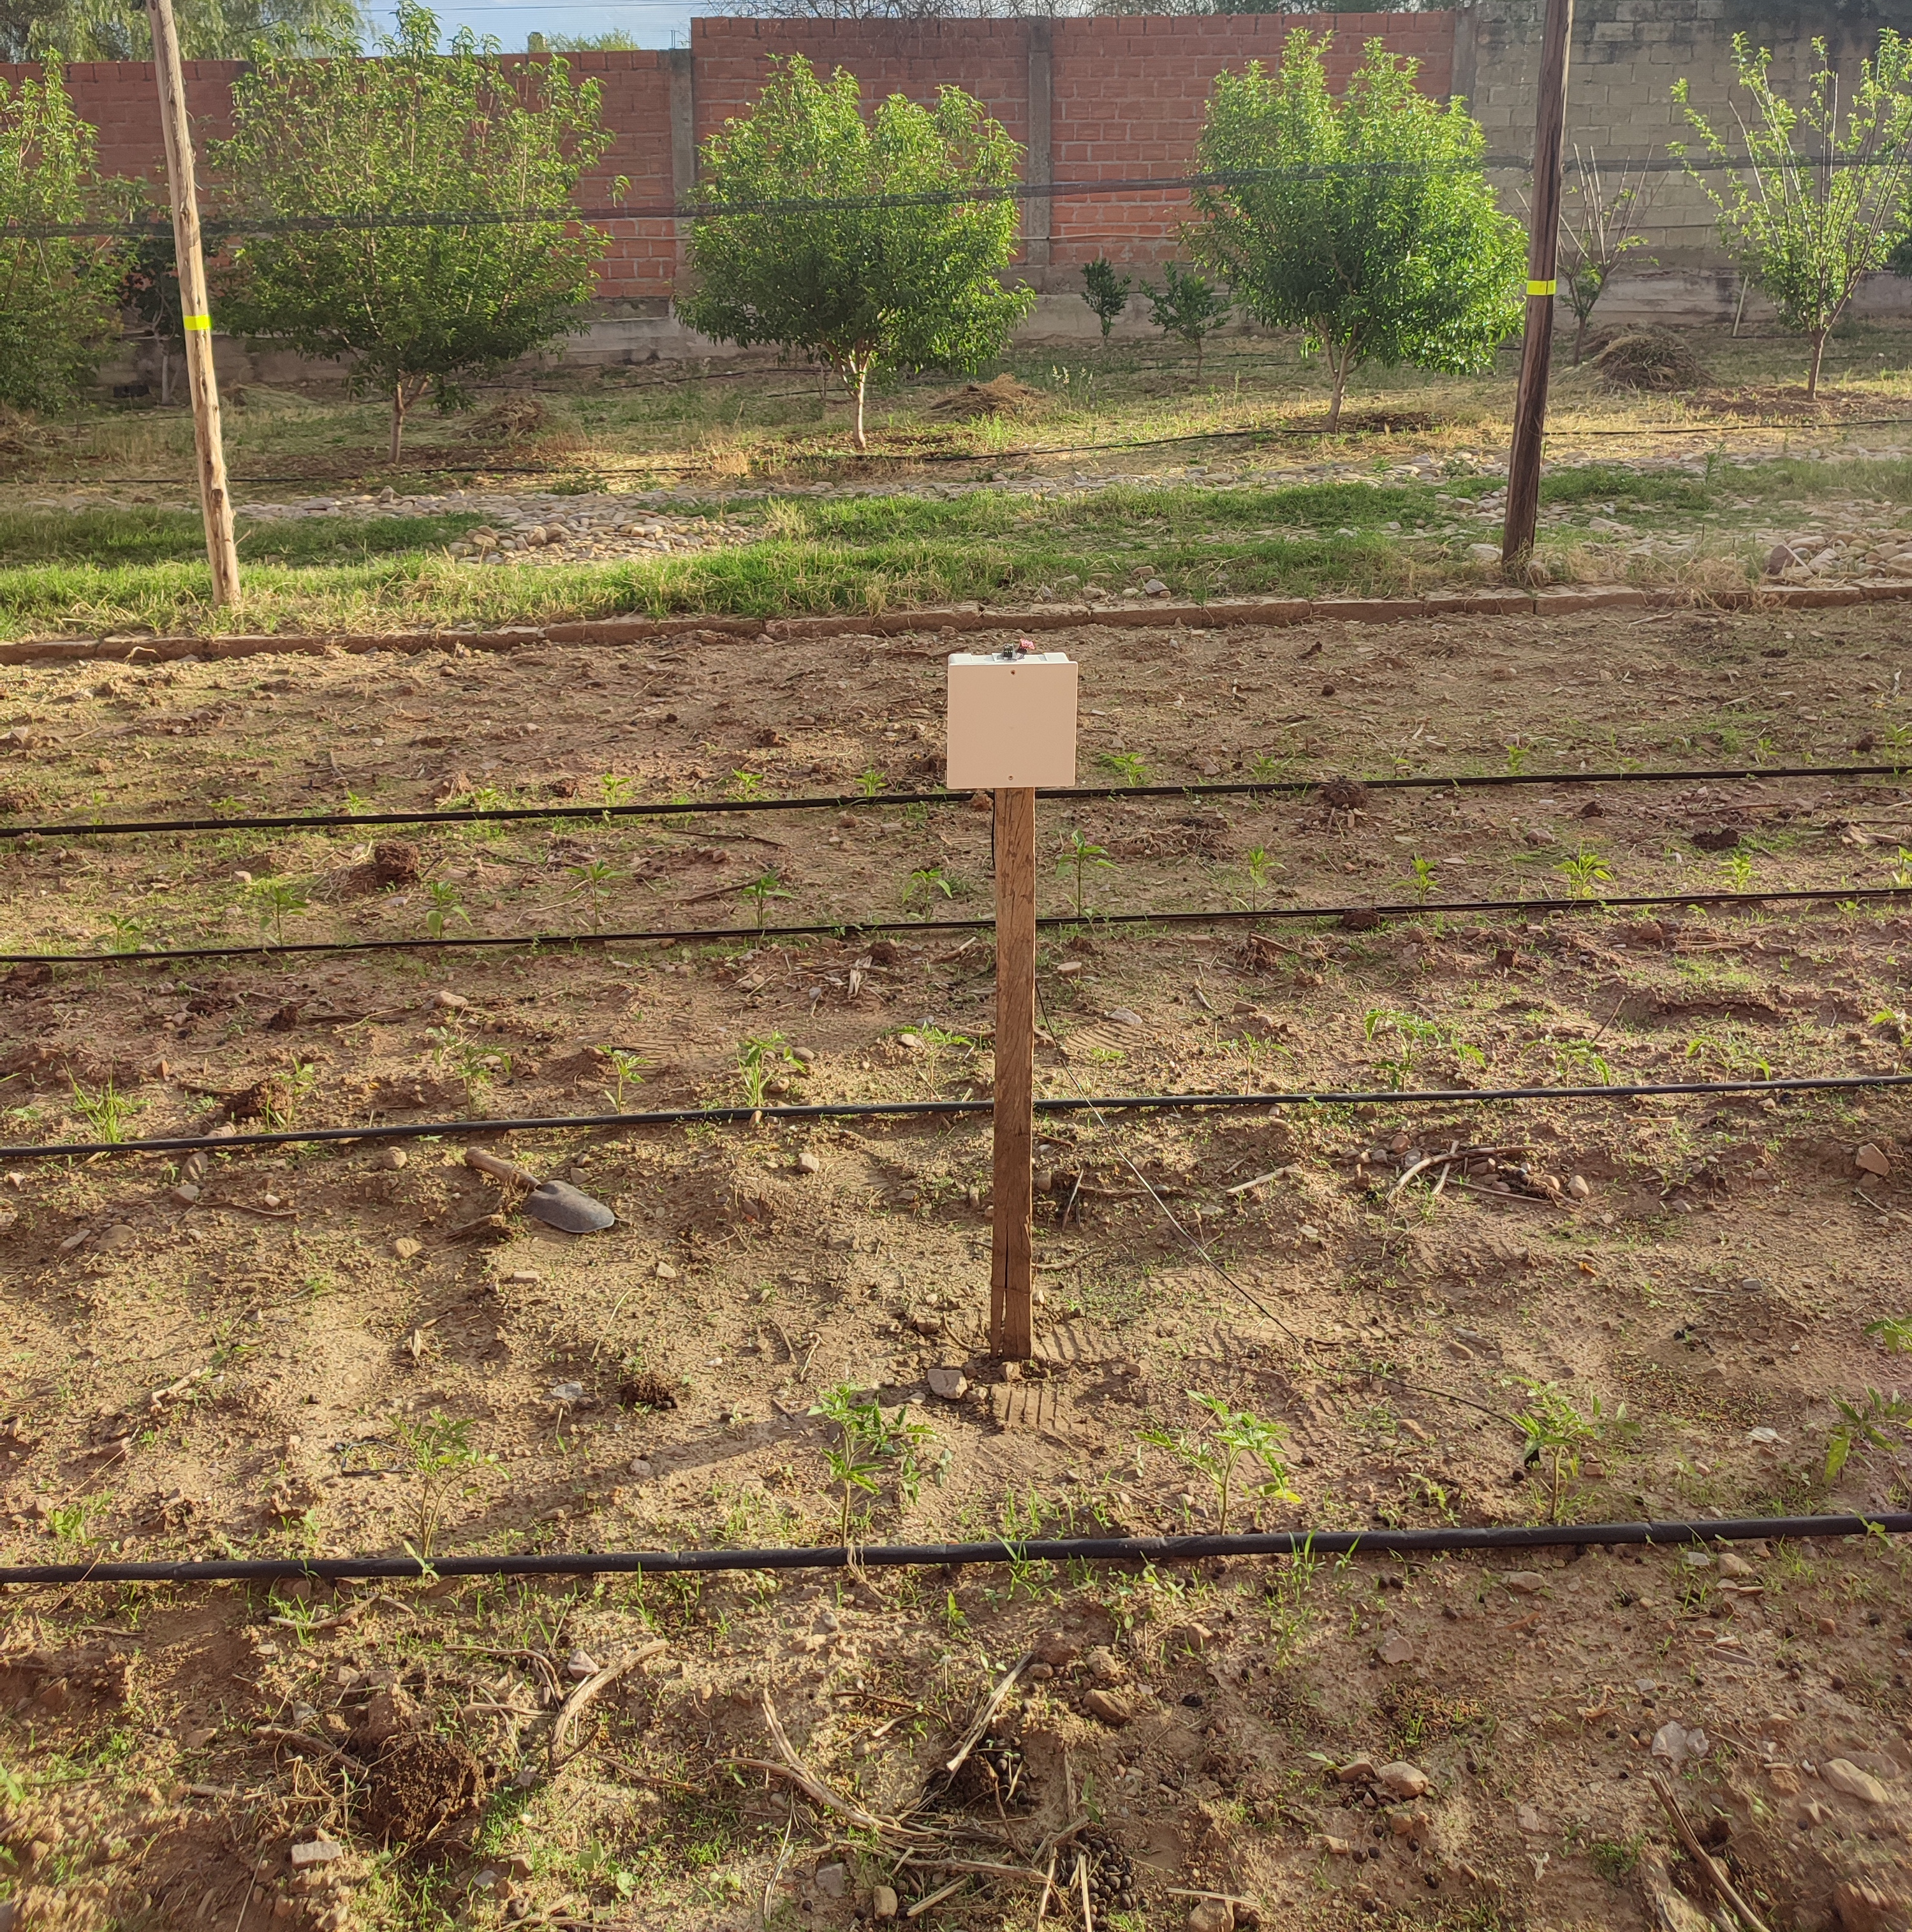
\includegraphics[width=5cm, height=5cm]{./Figures/protopito_sol.jpg}
  \caption{Condiciones ambientales prueba 1.}
    \label{fig:Condicionales ambientales prueba 1}
\end{figure}

En la figura \ref{fig:Lectura tierra seca tb} se muestran los resultados de la lectura de los sensores en las condiciones anteriormente mencionadas. Se tiene una lectura de humedad de suelo de 19\%, radiación moderada de 5UV y temperatura ambiente del 32\textcelsius.

\begin{figure}[h!]
  \centering
    \includegraphics[width=\linewidth, height=7cm]{./Figures/tb_prueba1.png}
  \caption{Panel de visualización con las lecturas obtenidas en la prueba 1.}
    \label{fig:Lectura tierra seca tb}
\end{figure}

\subsubsection{Prueba dos}
Para la prueba dos se tenian las siguiente condiciones:
\begin{itemize}
  \item Tierra con humedad
  \item Temperatura moderada
  \item Horario de la lectura: 8 a.m
\end{itemize}
En la figura \ref{fig:Humedad en el suelo} se puede apreciar las condiciones ambientales en el momento de la prueba.
En la figura \ref{fig:Humedad alta ThingsBoard} se muestran los resultado de la lectura. Como resultado tenemos: humedad del suelo del 75\%, radiación baja de 2UV, humedad ambiente de 54\% y temperatura ambiente de 23\textcelsius.

\begin{figure}[h!]
  \centering
    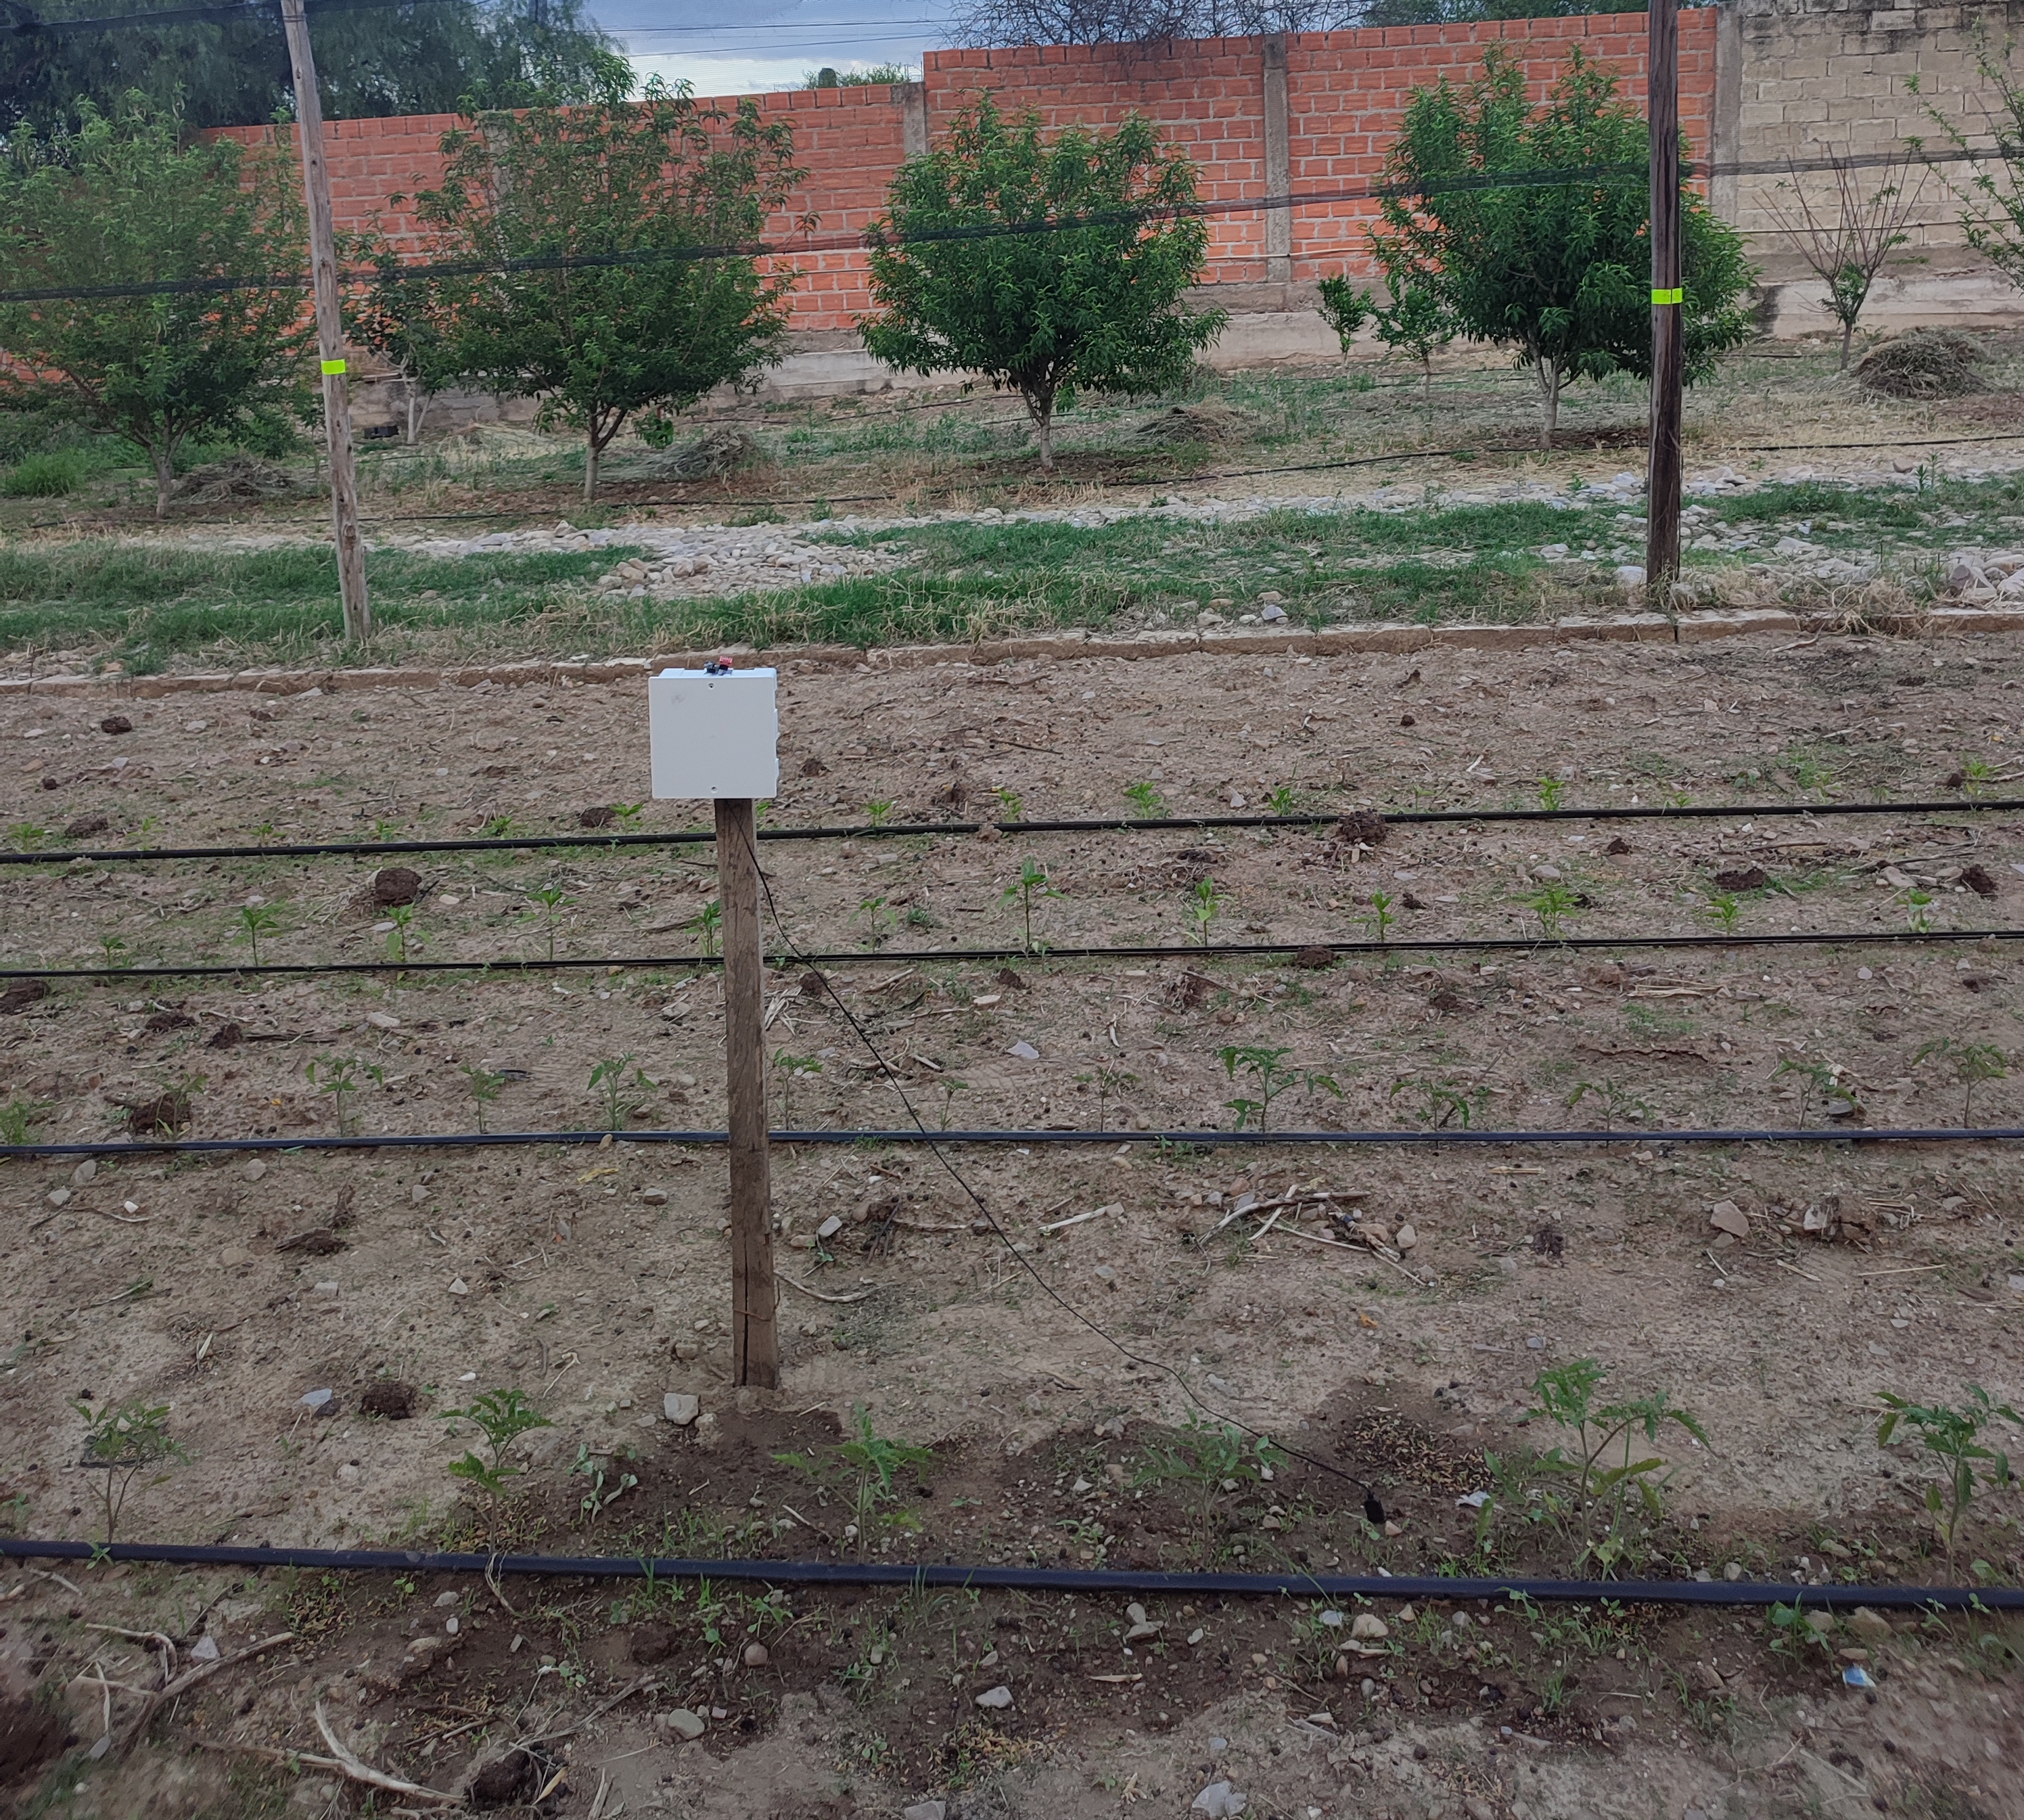
\includegraphics[width=5cm, height=5cm]{./Figures/prototipo_con_humedad.jpg}
  \caption{Condiciones ambientales prueba 2.}
    \label{fig:Humedad en el suelo}
\end{figure}

\begin{figure}[h!]
  \centering
    \includegraphics[width=\linewidth, height=7cm]{./Figures/humedad_alta_tb.png}
  \caption{Panel de visualización con las lecturas obtenidas en la prueba 2.}
    \label{fig:Humedad alta ThingsBoard}
\end{figure}

\subsection{Prueba del envío de datos al broker MQTT}
Una de las tareas más importante del firmware, es la del manejo de la comunicación con el servidor. Para verificar el funcionamiento de esta tarea, tenemos que ver la secuencia de comandos que manda el microcontrolador al módulo de comunicación.
Para realizar esta prueba se conectó un convertidor UART a USB al conector de depuración que tiene nuestro dispositivo.
En la figura \ref{fig:secuencia de comandos shell} podemos observar toda la secuencia de comandos que realiza el firmware para realizar el envío de datos a la plataforma IoT. Primeramente se envía el comando que verifica si el módulo está activo, luego se configura el apn de la red, se conecta al broker MQTT, se publican los datos y finalmente, se realiza el proceso de desconexión del broker.

\begin{figure}[h]
  \centering
    \includegraphics[width=12cm, height=9cm]{./Figures/secuencia de comandos shell.png}
  \caption{Comandos para enviar datos al broker MQTT.}
    \label{fig:secuencia de comandos shell}
\end{figure}

\subsection{Prueba de envio de alarmas por SMS}
El objetivo de esta prueba es verificar el funcionamiento de la alarma que monitorea la humedad del suelo.
Cuando la humedad del suelo baja por debajo del rango permitido. El firmware manda un SMS al usuario con el mensaje de "Humedad de suelo muy baja". En la figura \ref{fig:humedad menor} podemos ver que la humedad bajó de 10\% y en la figura \ref{fig:sms alarma} que se recibió el SMS de alarma.

\begin{figure}[h!]
  \centering
    \includegraphics[width=\linewidth, height=4.6cm]{./Figures/humedad_menor2.png}
  \caption{Humedad del suelo menor al 10\%.}
    \label{fig:humedad menor}
\end{figure}

\begin{figure}[h!]
  \centering
    \includegraphics[width=5cm, height=3.5cm]{./Figures/sms_alarma2.jpg}
  \caption{Recepción del SMS con el mensaje  de alarma.}
    \label{fig:sms alarma}
\end{figure}

\label{sec:pruebasHW}

